\section{Back End}
The back-end contains the code that deals with processing scene data, this block is decomposed into
two main blocks, the photon mapping block and the ray-tracing block, the photon mapping block is responsible
for the prepossessing step that creates the photon maps used to estimate the radiance. The ray-tracing stage
is responsible for computing the colour of each of the pixels in the output image, this will use the data
that was read into from the front end and the photon maps that were created by the photon map module. The
output of the ray-tracing block is sent to the front end which will use the data to present or save the final
image. Both the photon map generation and ray-tracing stages have been designed as pipelines with data being passed
between threads in a producer consumer pattern through thread-safe queues.

\subsection{Photon Emission and Photon Map Construction}
We further decompose the photon map generation into two stages, the photon emission stage which traces photons
through the scene and stores the point of absorption and the balancing stage which sorts the photons into
a data structure (left balanced tree) that facilitated efficient storage and searching.
The reason for the balancing stage is that the distribution of the photons in the map is unlikely to be
optimal \cite{JensenBook}.

The construction of the photon map can be computationally expensive when a high number of photons are
requested to be created, in order to improve the performance of this stage multiple threads are created
that are responsible for emitting a proportion of the photons in the final photon map, the number of threads will be
set in the front end and is configurable by the user to suit the machine that the system is being run on.

Each of the threads will trace a photon through the scene, at each diffuse interaction it will write the
photon to the output queue, the photon will then be reflected to continue the photon map construction.

The next stage in the pipeline reads photons from the queue, this will continue until each of the threads
has signalled that they have completed processing the photons, once all of the threads have been completed the
the list of photons will be transferred into the photon map as a left balanced tree.

\begin{figure}
\centering
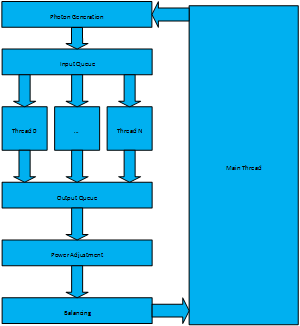
\includegraphics{./images/photon_threading.png}
\caption{Photon map generation}
\label{fig:photon_generation}
\end{figure}

\subsubsection{Multiple Photon Maps}
During the construction of the photon maps a choice must be made as to which of the photon maps the photon
should be placed in, this requires additional information to be passed from the emission thread, this information
will describe the path that the photon has taken, this will in essence be an implementation of the path notation
that is commonly used to describe the path of a photon, in this case all paths will be stored in the global photon
map (\textbf{L(S\textbar D)$^+$D} in the path notation),only specular paths are stored in the caustic photon map
as these are the paths that contribute the most to the focusing effect of caustics (\textbf{LS$^+$D}) note that
we have no eye component as the photons are only traced to diffuse surfaces.


\subsection{Ray-tracing}
As can be seen from Figure~\ref{fig:design_blocks} the ray-tracing module contains multiple threads, each of these
threads trace a subset of the pixels in the image and run independently to each other, this is possible due
to the inherent parallelism in the photon mapping algorithm. This stage in the system will perform ray-tracing
as described by Shirley \cite{shirley-dist}, for each intersection found during the running of the system the photon
maps created during previous stage will be used to estimate the radiance of the point in order to estimate the
true illumination at the point factoring in the global effects.

\begin{figure}
\centering
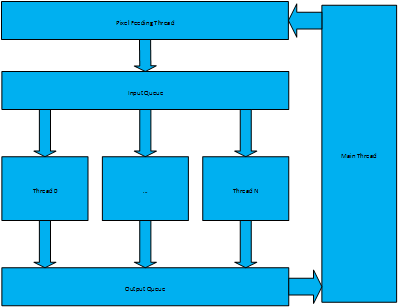
\includegraphics{./images/pixel_threading.png}
\caption{Ray-tracing architecture}
\label{fig:pixel_generation}
\end{figure}

The architecture of the ray-tracing block shared many similarities with that of the photon emission stage,
it is also a pipeline, there is a threads that inputs each pixel in the output image to a queue, this queue
is in turn read by one of multiple threads that perform photon mapping for a ray emitted through the pixel,
multiple rays are generated for each pixel performing distribution ray-tracing, the colour of the pixel is
then written to an output queue that will be read by the main thread in order to send the pixel values to
the front end to be presented to the user.

\subsection{Objects}
Much of the ray-tracing algorithm that is performed on each of the
objects in a scene is the same, for example finding a refracted
ray is only dependant on the surface normal at a point of intersection
for this reason the system abstracts any object that can be intersected
must implement certain functions, this is a form of object orientation.

\subsubsection{Materials}
In order to determine the path of the photons that are emitted and determine the colour of the pixels when
performing ray-tracing we require a description of the reflectance of the surface, we have decided to model
perfect diffuse surfaces and perfect specular reflectance and transmission, we store this information
as coefficients $\sigma_d, \sigma_r, \sigma_t$, each of which contain a red, blue and green components, 
participating media also require two more coefficients, the absorption and scattering coefficient again
with three colour components.

\subsection{Shading}
Each thread is responsible for performing that shading at the intersection of eye rays, for specular reflection
and transmission this results in an additional ray-trace be performed to determine the shading colour, for diffuse
surfaces a direct illumination calculation is performed, additionally the photon map is queried to determine
the indirect lighting. For participating media, the radiance is calculated by performing by a ray-marching
procedure.
